\chapter{Background and Related Works to the Embracing Sphere}
    This chapter establishes fundamental concepts related with Embracing Sphere by covering in-depth environmental storytelling, acoustics and haptics. The chapter aims to investigate artworks and video games chosen for their relation to the Embracing Sphere on both conceptual and practical levels.\par
    \section{Environmental Storytelling and Developments in Virtual Environments}
        Discussions about environmental storytelling as a term in narratology dates back not so long ago. First defined in 2000 by Don Carson, a former theme park designer for Walt Disney Imagineering, argues that in themed environments “the story element is infused into the physical space a guest walks or rides through”\cite{Liminal_Space_Between_Embedded_and_Emergent_Narrative}. During his work in theme park train rides or video games, his objective to tell a story through the experience of traveling through a real or imagined physical space\cite{Lessons_Learned_from_the_Theme_Park_Industry}.\par

        These discussions later developed into a game design discourse as concept of "story versus play", "ludology vs narratology\cite{Hamlet_on_the_Holodeck}" within transmedia storytelling\cite{Jenkins_Shall_We_Play}. Jenkins argues that the story becomes richer and more complex, as the audience is given more opportunities to engage with the narrative.\par

        Although the transmedia storytelling directs something else (a process where integral elements of a fiction get dispersed systematically across multiple delivery channels\cite{Jenkins_Transmedia}) a discussion of the narrative potential of video games supported attempts to create narrative spaces in virtual environments\cite{Liminal_Space_Between_Embedded_and_Emergent_Narrative}.\par

        \subsubsection{Case Study: Journey}
            \emph{“Like a religious ritual of passage, it is not the spiritual narrative’s plot, but rather the poignant symmetry between its metaphorical meaning. The embodied experience of performing the movements it channels, that makes this narrative effective. Journey makes zero use of language and relies entirely on the experience of movement to tell its story\cite{Game_Movement_as_Enactive_Focalization}\cite{Narrative_Geography}.”}\par

            \begin{figure}[H]
                \centering
                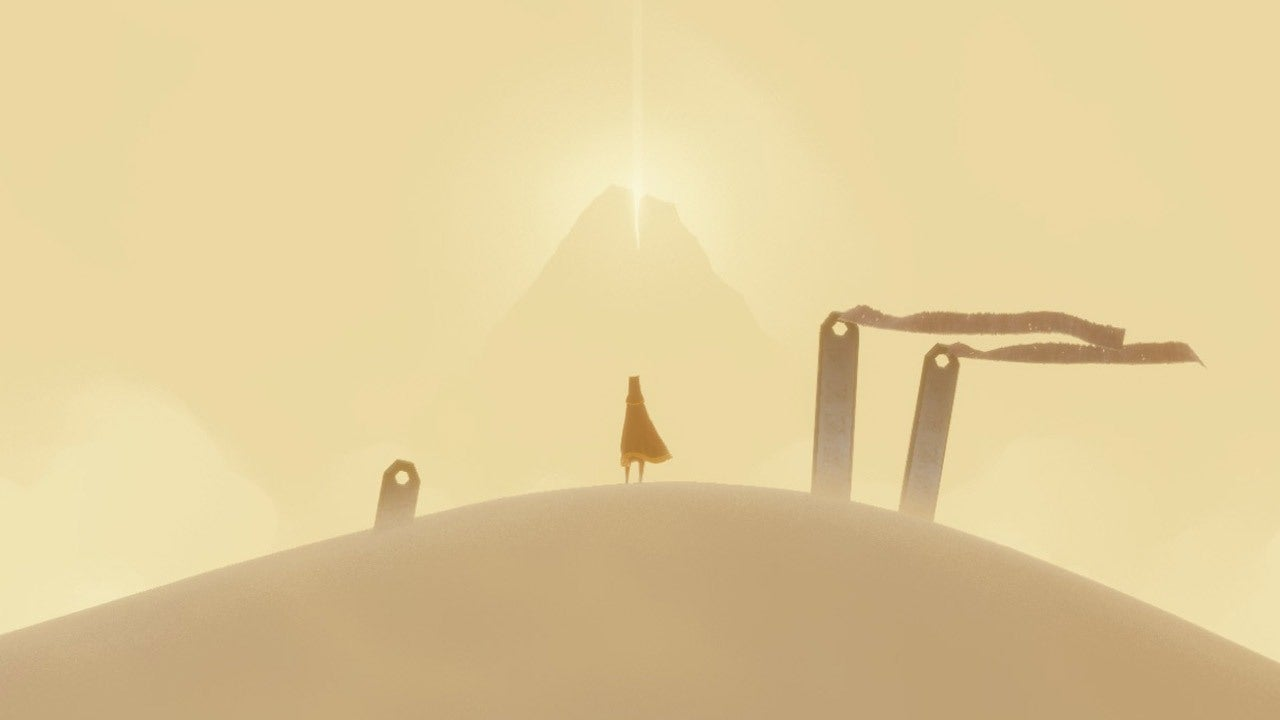
\includegraphics[width=0.8\textwidth]{images/journey.jpg}
                \caption{A visual from the game called Journey released in 2012 by Thatgamecompany and Santa Monica Studio.}
                \label{fig:JOURNEY}
            \end{figure}

            Environmental storytelling in video games done by staging the game world so that the arrangement of objects, scenery and audio cues naturally conveys story to the player\cite{BioShock_Infinite}.\par

            Journey is a video game has critic focus on exploration and a great, well awarded (Journey won several "Game of the Year" awards from different organizations) example for environmental storytelling. The game accomplishes this narrative success mostly by not relying any use of linguistics or semantics.\par

            In Journey, the player controls a figure starting in a vast desert, traveling towards a mountain in the distance in a multiplayer environment, which means you as a player can meet interact with other players on the same journey. The challenge is, players cannot communicate via speech or text and cannot see each other's names until after the game's credits.\par

            Players have basic navigational controls like walking, jumping, sliding on the dunes and ability to emit a wordless shout to another. The length and volume of the shout depends on how the button is pressed.\footnote{Journey shout example: \url{https://youtube.com/clip/UgkxMXBXc4aZmHuOL2f3PUoEVQ57Og5Suyks/}}\par

            Through the players path in Journey, one distinct element always catches eye. The big shining mountain peak in the horizon, pictures an unspoken, ultimate goal or a direction for our journey. Each player trying to reach the peak either by helping each other or going this path individually.\par

            \begin{figure}[H]
                \centering
                \includegraphics[width=0.8\textwidth]{images/journey_mountain.png}
                \caption{The mountain in the video game, Journey.}
                \label{fig:JOURNEY_MOUNTAIN}
            \end{figure}

            The subtractive design of Journey's game environment forcing player to focus on the environment all the time. Directing to consume story through cryptic glyphs, symbols and figures carved into the walls, artistically placed in the game environment.\par

            By collecting these symbols, players gain more movement ability to explore deeper in the game. This mechanic also shown in diegetic way with a scarf wrapped around the player characters head. The scarf is giving information about your energy left to jump and fly around like the fuel in your tank or stamina left. The scarf grows as you progress through the game by picking up collectible symbols.\par

            \begin{figure}[H]
                \centering
                \includegraphics[width=0.8\textwidth]{images/journey_scarf.png}
                \caption{The player's scarf in the Journey.}
                \label{fig:JOURNEY_SCARF}
            \end{figure}      

            In Journey, the narrative aspect of the non-linguistic communication and the movement through the designed space, generates the story. The player reconstructs the story by interpreting different objects in ruins, interacting with the others and initializing events embedded in the game environment.\par

            Video game in that sense has one characteristic feature, which is their spatiotemporality. In comparison to other multimedia mediums like cinema which is purely temporal sequences, we can view video games narrative as a blend of the temporal and the spatial\cite{Liminal_Space_Between_Embedded_and_Emergent_Narrative}.
        \subsection{Existing Methods in Different Mediums}
            Environmental storytelling is not entirely specific to video games. First in theaters then later adopted in screenplay, there is a French term called "mise-en-scene" in literal translation "putting into the scene". Mise-en-scene describes the arrangement of scenery, props, lighting and other visual elements to support the story. Filmmakers and production designers use settings to provide backstory and mood. For example, a character’s cluttered apartment, lit by a flickering lamp, can imply their personality and situation before they even speak. In cinematic terms, every object in the frame is there by choice to serve the narrative.\cite{Mise_en_scene}\par
        
            Details like wall posters, broken objects or photographs can signal past events. A close-up of a train ticket on a nightstand might hint where a character planned to go. In film theory, such embedded clues function like visual foreshadowing. Viewers can pick up these details either consciously or subconsciously. Production designers and directors use every element of mise-en-scene to make the environment feel lived-in and story-rich.\par
            
            For the comparison between cinema and video games, we can broadly categorize video game narrative broadly into 2 categories: "embedded narrative", which follows pre-authored contents as temporal narrative sequences that still exist without audience action and "emergent narrative" which is directly linked with audiences meaningful action, exploration and interaction with the virtual environment\cite{Liminal_Space_Between_Embedded_and_Emergent_Narrative}. Cinema, doesn't have emergent narrative due to its fixed media characteristics. According to Natalia A. Bracikowska, environmental storytelling exist in liminal space between embedded and emergent narrative\cite{Liminal_Space_Between_Embedded_and_Emergent_Narrative} and this aspect of environmental storytelling opens a pretty viable path to convey multi-branched story bits for the audience.\par
            
            Across interactive media, game design and film theory, environmental storytelling is a shared strategy to embed narrative in the space itself. In all domains, meaning is conveyed indirectly. Games and interactive media emphasize the user’s role in uncovering that meaning players must explore and investigate to “do the work” of interpretation. In contrast, films present a fully authored scene but still rely on designed space to impart story context. There is a common goal to see, which is to make every detail of the world serve the story.\par
        \subsection{Auditory Environmental Storytelling}
            \emph{"Sound is a integral part of every performative and aesthetic experience with an artifact. Yet, in design disciplines, sound has been a neglected medium, with designers rarely aware of the extent to which sound can change the overall user experience."\cite{Sonic_Interaction_Design}}

            According to Stefania Serafin, humans are sensitive to sounds arriving from anywhere within the environment whereas the visual field is limited to the frontal hemisphere, with good resolution limited specifically to the foveal region. Therefore, while the spatial resolution of the auditory modality is cruder, it can serve as a cue to events occurring outside the visual field-of-view\cite{Sonic_Interaction_in_Virtual_Environments}. Therefore effective auditory environmental storytelling relies on a sophisticated understanding of how different sound elements function individually and collectively to shape the user experience.\par

            The concept of "presence" and "immersion" highly relates with this subject in perspective of auditory domains characteristics on fully spherical perception and cognition.\par

            Immersion is a studied in multiple different field such as film, video games and music. It is a subject that can have different meaning depending on the context of the field of study\cite{Sonic_Interaction_in_Virtual_Environments}. Immersion is a metaphorical term that derived from the physical experience of being surrounded. In Janet H. Murrays words, "being submerged in water"\cite{Hamlet_on_the_Holodeck}. 

            Presence on the other hand is a term that used in much broader sense. According to Lombard and Ditton, presence described as the feeling of “being there” in a mediated environment, even though the experience is happening through a screen or device. Presence can occur in different forms, such as feeling physically in a place shown on screen, socially connected to others through media, or involved in an environment that reacts to one’s actions\cite{Concept_of_Presence}.

            By understanting how we naturally interact with the world, how we interpret information provided by sensory stimulations, we can apply this understanding to enhance and elevate the immersion and presence in our intended mediums.\par

            Therefore auditory stimulation by its nature, envelopes a lot of human sensory aspects. It is explicitly useful for its spatiotemporal narrative capabilities. With a case study that explores a video game called Return of the Obra Dinn we can have deeper understanding on auditory environmental storytelling.\par
        \subsubsection{Case Study: Return of the Obra Dinn}
            Return of the Obra Dinn, is a adventure-puzzle video game developed by Lucas Pope in 2018. In the backstory of the game, The Obra Dinn, a merchant ship missing for five years, has reappeared off the coast of England with no known surviving crew or passengers. Players task is to determine every crew members fate, including their names, how they met their fate, who or what killed them and if anybody alive, where are they?\par

            \begin{figure}[H]
                \centering
                \includegraphics[width=0.8\textwidth]{images/ship_02.png}
                \caption{A visual of the ship deck from the game called, Return of the Obra Dinn released in 2018 by Lucas Pope.}
                \label{fig:SHIP}
            \end{figure}

            Players can hop onto the Obra Dinn and navigate on the main deck. The main mechanic portrayed with a latin phrase, "Memento Mortem", a mystical pocket watch that allows the investigator to witness the final moments of any corpse discovered aboard the ship.\par 

            \begin{figure}[H]
                \centering
                \includegraphics[width=0.3\textwidth]{images/pocketwatch.png}
                \caption{A visual of the pocketwatch in Return of the Obra Dinn.}
                \label{fig:POCKETWATCH}
            \end{figure}

            When player approach to a remaining of a crew member the pocket watch can be activated and it triggers a sequence that includes 2 parts: first, an audio snippet right before the event happened, secondly a static, frozen explorable visual tableau of the event that results the death scene.\par

            \begin{figure}[H]
                \centering
                \includegraphics[width=0.8\textwidth]{images/ship.png}
                \caption{A visual of the of a remaining of crewmember in Return of the Obra Dinn.}
                \label{fig:CREWMEMBER}
            \end{figure}

            The crew member shown in the \ref{fig:CREWMEMBER} is our first case to solve in this adventure-puzzle game. As we interact with the body remain, a musical cue transport us to the past and we hear an audio snippet\footnote{Return of the Obra Dinn, first audio snippet: \url{https://youtu.be/UXC6Sjsedcg}} which transcription is like that:\par
            \emph{
                \newline
                - "Captain! Open the door..."\newline
                - "Kick it in!"\newline
                - "...lest we break it down... ...and take more than those shells."\newline
                - "You bastards may take... ...exactly what I give you.[DOOR OPENING AND GUN SHOT]"\newline
                }

            \begin{figure}[H]
                \centering
                \includegraphics[width=0.8\textwidth]{images/static_scene.png}
                \caption{A visual the static scene of Return of the Obra Dinn.}
                \label{fig:STATICSCENE}
            \end{figure}            

            At the point \ref{fig:STATICSCENE} we have enough sensory cues to solve at least 1 crew members identity which is the Captain himself and we have enough hints to define how this crew member died. Because according to the auditory cues one crew member calls "Captain!" and knocking the door in anger. The other crew member is suggesting to kicking the door and forcefully get into the room. The only person we hear behind door opens it and shoots one of the rebellious crew member immediately.\par

            \begin{figure}[H]
                \centering
                \includegraphics[width=0.8\textwidth]{images/crewmembers.png}
                \caption{An illustration of crew member of the Obra Dinn.}
                \label{fig:SHIPCREW}
            \end{figure}   

            While the visual scene is frozen, the audio snippet captures the ambient soundscape of that specific moment and location. This ambient layer logically contributes to differentiating scenes and grounding the abstracted visual tableaus in a more tangible sense of place. It is in my perspective, a well done auditory environmental storytelling.\par           

            My experience with this video game was a great inspiration for Embracing Sphere after all. It showed me the possibility of environmental storytelling is indeed strong and it has benefits for spatiotemporal story cases.\par

            After covering necessary perspective from narratology and video game studies, sound and perception are going to be investigated in more detail, specifically acoustics and psychoacoustics subjects within the next subchapter.
    \section{Room Acoustics}
            \emph{"Sound is something most people take for granted. Our environment is full of noises, which we have been exposed to from before birth. What is sound, how does it propagate and how can it be quantified\cite{Acoustics_and_Psychophysics}?"}\par 

            The purpose of this subchapter is to introduce fundamental knowledge ground for room acoustics and describe the usage of room impulse responses in the Embracing Sphere context.\par
        \subsection{Definitions for Room Acoustics}
            Sound is simply a mechanical disturbance of the medium. Medium in that context may be air, solid, liquid or other gas matters. Dependent on the mediums state, the sound can be propagated and while this propagation happens it interacts with physical objects and other sound waves. In room acoustics the interactions of the sound with the medium, basically can be listed as refraction, absorption, reflection and interference. Psychoacoustics is the study how humans perceive sound after all these interactions with the medium\cite{Acoustics_and_Psychophysics}.\par

            The heard sound, is the result of all these complex physical interactions in the place our ears are located.\par

            When sound moves through a room, its behavior is shaped by how it interacts with surfaces, mainly through absorption and reflection. Sound reflection occurs when sound waves hit a hard boundary and bounce back into space. In contrast, sound absorption is when a material takes in the sound's energy, which is converted into small amounts of heat through internal friction, reducing the amount of sound that reflects\cite{Acoustics_and_Psychophysics}. For example, a wooden surface absorbs more sound than a rough concrete one. These interactions, along with others like refraction and interference, collectively determine the acoustic character of a room.\par

            These interactions do not occur in isolation. They collectively define the complex behavior of sound waves and their propagation within the room. Each time a sound interacts with a surface in a room it loses some of its energy due to absorption and reflection. The time that it takes for a sound to die away at any given time in a room is called the reverberation time.\par

            Reverberation time is an important aspect of sound behavior in a room. Mentioned different absorption coefficient values in different materials and frequencies shapes the perception of the room. If the sound dies away very quickly, we perceive the room as being “dead” or if the sound dies away very slowly, we perceive the room as being “live”. To calculate reverberation times there is a simple formula known as the “Sabine formula”, named after its developer Wallace Clement Sabine\cite{Acoustics_and_Psychophysics}.\par 
            $$RT_{60} = \frac{0.161 \cdot V}{A}$$
            \begin{itemize}
                \item RT60: This is the reverberation time in seconds. It's defined as the time it takes for the sound pressure level in a room to decrease by 60 decibels (dB) after the sound source has stopped\cite{Room_Acoustics}.
                \item 0.161: This is a constant. Its units are seconds per meter (s/m). This constant is derived empirically and is based on the speed of sound in air at a typical room temperature.
                \item V: This represents the volume of the room in cubic meters. Calculated by multiplying the length, width and height of the room.
                \item A: This is the total sound absorption of the room in Sabins. It's calculated by summing the absorption of all surfaces in the room. The absorption of each surface is found by multiplying its surface area in square meters by its sound absorption coefficient at a specific frequency.
            \end{itemize}

            According to the Sabine formula, reverberation time depends on the volume, surface area and the average absorption coefficient in the room. However, the absorption coefficients of real materials are not constant with frequency. This difference in absorption strength in different frequencies changes heard timbre of the room as the sound in the room decays away. Apart from being useful, Sabine formula has assumptions for speed of sound and static response of the reflective materials in the room. To more accurately measure reverberation time, another method called room impulse response capturing was introduced in 1964 by M. R. Schroeder \cite{New_Method_Measuring_RT}.\par

            This method uses tone bursts (or filtered pistol shots) to excite the enclosure (room). The captured smooth decay curves resulting from the new method improve the accuracy of reverberation time measurements and facilitate the detection of non-exponential decays\cite{New_Method_Measuring_RT}.\par

            These impulse response recordings can be used later to reconstruct a virtual environment with the same reverberation curves as captured room with a mathematical operation called convolution. An anechoic (no reflections) sound is convolved with an RIR and this mathematical process applies the room's acoustic snapshot to the sound. The convolution effectively embeds the reflections and reverberation captured in the RIR to the original sound.\par
        \subsection{Room Impulse Response Measurement Methods}
            \emph{"Between stimulus and response there is a space. In that space is our power to choose our response. In our response lies our growth and our freedom."\cite{Sonic_Interaction_in_Virtual_Environments}}

            The quote above is highly controversial because it has been referred to an Austrian neurologist and psychologist, Viktor Frankl by Stephen R. Covey in his book called The Seven Habits of Highly Effective People but quote that referred to Frankl's book, Man’s Search for Meaning hasn't got any line that includes the quote. Although I wanted to share this quote as a poetic mood setter for this chapter.\par

            From an artistic perspective, Embracing Sphere refers to this metaphorical concept of relation between stimulus and response of space. Either directly or metaphorically it is powerful representation in spatial perception. Embracing Sphere is about creating an environments/spaces that are capable of telling stories. These spaces should contain both stimulus and response. Although in Embracing Sphere, audience doesn't have power of choice, space has that power because I view the space as an actor that has a lot to tell. The response of the space, grows and establish its freedom.\par

            Acoustics, mathematics, methodologies around it can be covered so deep in details but in the end all of these descriptions and formulas exist in my research to support my artwork to understand the background and design choices of the Embracing Sphere. Therefore RIRs are important in my artwork to give acoustic and spatial context to the audience. It is useful to render the depth and the aural character of the environment into audio content.\par

            In previous sections we covered room impulse response description in surface level. It is a captured audio file that contains acoustics space characteristics such as frequency changes, reverberation decay and length.\par

            There are several practical ways to capture RIR of a room. The easiest one is popping a balloon in the desired room and recording the balloon pop. This method is practical but not much accurate and it is not easy to recreate again because every balloon pop sound parameters can be differ in frequency-wise\cite{RIR_Swept-Sine_Technique}. The more accurate method is sine sweep technique\footnote{A sine sweep IR capture example: \url{https://youtu.be/1egKAtC16e8?feature=shared}}, which includes 1 reference sine wave sweep audio (5-10 seconds long) that starts from 20Hz and sweeps every frequencies until 20kHz\cite{Auditory_Perception_of_Sound_Sources}. In this method the room is acoustically excited by this sine wave and with a microphone the room response recorded then processed with a mathematical process called deconvolution that extracts RIR with subtracting reference sine sweep from reverberant recording.\par

            \begin{figure}[H]
                \centering
                \includegraphics[width=0.8\textwidth]{images/IR_Capture_Balloon_Pop.png}
                \caption{A visual from a recording session for capturing room impulse response in an old house in Balat, Istanbul.}
                \label{fig:IR_BALLOON}
            \end{figure}            

            The visual in \ref{fig:IR_BALLOON} is a recording session in 2021 when I was working as an audio designer in a company called Vadi Sound. In that frame we were capturing RIR with balloon popping in an old house in Balat, Istanbul. The house specifically interesting for capturing RIR because it was one of the few historical wooden houses remain in the Istanbul from early Turkish Republic times. In that situation we hadn't got any high quality full range speaker to excite the room so we choose to pop a balloon at several places in the room to capture as many different positions RIR.\par

            \begin{figure}[H]
                \centering
                \includegraphics[width=1\textwidth]{images/IR_Capture_Sine_Sweep.png}
                \caption{A visual of a RIR capturing session in a studio using sine sweep method. Retrieved from Audioease website \url{https://www.audioease.com/altiverb/browse.php}}
                \label{fig:IR_SINE}
            \end{figure}

            An RIR capturing session that using sine sweep method can be seen in the figure \ref{fig:IR_SINE}. The specific setup uses 2 omnidirectional microphone positioned in the A/B stereo miking technique (a well known stereo miking technique in ambience recordings.)\cite{Sound_Reinforcement} and 1 binaural microphone to capture studio room impulse response.\par

            \begin{figure}[H]
                \centering
                \includegraphics[width=0.6\textwidth]{images/Room_RT.png}
                \caption{An illustration of raytracing of a sound in a close environment. Drawn in AMROC website \url{https://amcoustics.com/tools/amray}}
                \label{fig:IR_RAYTRACE}
            \end{figure}

            Either method works in basic principle shown in the figure \ref{fig:IR_RAYTRACE}. A source that exciting the room and a capturing point that captures the room's acoustic character. From an artistic or design perspective we can see this process as taking an auditory snapshot of the room.\par

            \begin{figure}[H]
                \centering
                \includegraphics[width=1\textwidth]{images/IR_Comparison.png}
                \caption{Plotting of RIR files of 2 distinct spaces, a small room and The Hagia Sophia (Plotted with matplotlib and librosa in python).}
                \label{fig:IR_COMP}
            \end{figure}
            
            
        \subsection{Convolution in Math and Digital Audio}
            Convolution is a mathematical operation that combines two functions to produce a third function. This new function expresses how the shape of one function is modified by the other. In simple terms, convolution tells us how one signal changes when it passes through a system described by another signal. The convolution algorithm is often interpreted as a filter, where the kernel filters the feature map for certain information\cite{Deep_Learning_Core_Concepts}.\par

            We can say that convolution is fancy multiplication\cite{Guide_to_Convolution}. It is important in physics and mathematics as it defines a bridge between the spatial and time domains and the frequency domain through the convolution theorem. Convolution is essentially used in computer graphics, digital signal processing and lately in machine learning algorithms.\par
            $$(f \ast g)(t)=\int_{-\infty}^{\infty} f(\tau) g(t-\tau) d \tau$$
            The above formula is the formal definition of convolution operation. Instead of starting a calculus lecture, we can present a metaphoric example to deepen our understanding:\par

            Let's say you are running a restaurant. In this restaurant you have a fixed menu and your kitchen uses 2 eggs for one meal. In monday rush hour, 10 meals are ordered in the first hour, 11 in the second, and 12 in the third. How many eggs did you used? It's simple multiplication. 
            $$(2\cdot10)+(2\cdot11)+(2\cdot12)=66$$
            The answer is 66 but in Tuesday your chef added a dessert that requires an egg to make. Desserts are getting served after 1 hour of each meal. How many eggs you use for each hour? This is now a complex problem because the eggs amount overlaps after first hour.

            First hour is simple you prepare initially 10 meals with 2 eggs each. 
            $$2\cdot10=20$$
            Then the next hour you have to prepare 11 meal but also 10 desert for the visitors from first hour.
            $$(2\cdot11)+(1\cdot10)=32$$
            The third hour after your last visitors came you have to prepare 12 meals and additional 11 desserts for the second hour visitors.
            $$(2\cdot12)+(1\cdot11)=35$$
            And you overtime for the last visitors and serving 12 desserts.
            $$1\cdot12=12$$
            To summarise all the details,\par
            \begin{itemize}
                \item The Input (Orders): [10 11 12]
                \item The Plan (First meal, next hour dessert): [2 1]
                \item The Result (Total eggs used per hour): [20 32 35 12]
            \end{itemize}
            This calculation is a high level example for convolution operation. In digital audio with the lists that has at least 44100 samples\footnote{The Nyquist-Shannon sampling theorem states that a continuous signal can be accurately reconstructed from its discrete samples when the sampling frequency exceeds twice the maximum frequency present in the original signal\cite{Digital_Audio_Theory}.} per second, much more convolution operations needed to convolve an input audio (input) and an impulse response(kernel).\par

            Convolution is a key tool for processing sounds. It is used to apply the characteristics of one sound (such as the acoustics of a room or the response of a speaker) to another sound (like a musical recording or a voice).\par

            Convolution is also used in digital filters, such as equalizers and effects and in spatial audio to simulate how sound arrives at the ears from different directions. For example, by convolving audio with a head-related transfer function (HRTF), we can make sounds appear to come from specific locations in three-dimensional space\cite{3D_Audio}.\par
        \subsection{Room Acoustics in Sound Art} Explain Alvin Lucier - "I Am Sitting in a Room" Process-based art, using the room's acoustics as both medium and subject, the iterative feedback loop revealing resonant frequencies.
    \section{Haptics and Perception}
        \subsection{Overview of Haptics}
            Within the human body, somatic system can be subdivided into three elements: kinesthetic, visceral and cutaneous. Kinesthetic sensation uses signals from proprioceptors in the joints, muscles and tendons to provide feedback to the brain on the position and forces within segments. Similarly, visceral sensation uses receptors in the abdomen. Cutaneous sensation consists of the combined response of four types of nerve endings in the skin\cite{Human_Response_to_Vibration}. The haptic system uses sensory information derived from mechanoreceptors embedded in the skin, muscles, tendons and joints\cite{Haptic_Perception-A_Tutorial}.\par

            Haptic interaction can be stimulated by different devices but such as thermal feedback and electro-vibration are outside the scope of this study. Therefore a vibrotactile device chosen for this research. These vibrotactile devices are similar to those of loudspeakers and voice coil actuators\cite{Audio-Tactile_Rendering}, allowing for conventional audio recording practices viable on haptic feedback content creation.\par

            \begin{figure}[H]
                \centering
                
\includegraphics[width=0.4\textwidth]{images/vibrotactile_bass-shaker.jpg}
                \caption{Voice coil actuator, vibrotactile device, Dayton Audio BST-1.}
                \label{fig:VCA}
            \end{figure}

            The sensory system is a network that enables your body to receive information from the environment and its own internal state, converting stimuli into signals for the brain to process. The human sensory system doesn't just process this sensory information as a single stream; it organizes it to answer fundamental questions about the environment\cite{What_vs_Where_in_Touch}. Research in sensory neuroscience suggests a fundamental distinction in how the brain processes sensory information framed as "what" an object (disturbance) is versus "where" it is located.\par

            How do you feel the difference between rough stone, resonant wood, or soft earth? This relates directly to identifying the "what" of the surrounding environment. The "where" pathway provides spatial information, helping us to understand the location of a stimulus in relation to our body and within the environment. The location of a distant explosion felt through the floor, related to identifying "where" information.\par

            As we are exploring environmental storytelling through audio-tactile stimulation, we can extend this framework with a third component: "how". This component can include "cause and effect" relations within our sensory perception and cognition. Where "what" and "where" components answer material and spatial questions, "how" components can answer temporal questions derived from the first two components. These questions will focus on a more interactive concept of "event" rather than static stimulation characteristics.\par

            This "what, where and how" taxonomy provides a conceptual tool for environmental storytelling, thus embedding temporal relations into the environment, moving beyond simple rumbles to convey specific information about an environment's materials, spatial layouts and past/ongoing events.\par

            \begin{figure}[H]
                \centering
                
\includegraphics[width=0.8\textwidth]{images/rumble_strips.jpg}
                \caption{A visual shows road rumble strips.}
                \label{fig:RUMBLE_STRIP}
            \end{figure}

            As shown in the \ref{fig:RUMBLE_STRIP} rumble strips designed to alert drivers by creating vibrations and noise when a vehicle goes out from its intended lane or crosses the edge of the road. Stimulation from a rumble strip side of the road not just indicating physical position or a road surface information, it's an immediate warning.\par

            The sensation isn't a random patch of bad road; it's a deliberately engineered, rhythmic pattern. This pattern connects the what (the ribbed texture) and the where (the edge of the lane) to create a temporal meaning: "You are currently in the process of making a mistake." The "how" pathway interprets this sequence as a cause-and-effect event, because you are drifting, you are feeling this vibration. In a structured narrative context, this type of haptic stimulation can be utilized for environmental storytelling.\par

        \subsection{Human Tactile Perception} Briefly cover human tactile perception (how we sense texture, vibration, impact).
        \subsection{Usage} Examples of haptics in HCI, VR/AR, accessibility and gaming.
    \section{Audio-Tactile Interaction}
        \subsection{Definition of Audio-Tactile Multi-Modal Interaction} Define audio-tactility and explain differences from other multi-modal systems.
        \subsection{Usage of Audio-Tactility in Media} Examples of systems or experiences integrating audio and haptics.